% !TEX options=--shell-escape
\documentclass[french]{article}
\usepackage{common}

\usepackage{minted}
\usepackage{minted,xcolor} % [cache=false] if minted acts out

\setminted[python]{style=colorful}
\author{Gabriel Belouze}

\title{Kernel methods in machine learning : Homework 3}
\date{2021-2022}

\begin{document}
\maketitle

In case embedded links are not clickable on \textit{Gradescope}, all links from this document reference specific code section of the repository \href{https://github.com/gbelouze/mva-kernel-hw3}{https://github.com/gbelouze/mva-kernel-hw3}.

\section{Exercice 1. Support Vector Classifier}

\begin{enumerate}
\item
    \begin{enumerate}
    \item From the Representer theorem we can express $f = \sum_i \beta_i K_{x_i}$. We also write for convenience $Y = \diag(y)$. Then the Lagrangian writes
    \[ \frac{1}{2} \beta^T K \beta + C \cdot \xi^T\mathbf{1} - \mu^T \xi
    + \alpha^T (\mathbf{1} - \xi - b\cdot y - Y K \beta)
    \]
    \item
    The Lagrangian is affine in $b$, which yields the condition $\alpha^Ty = 0$ for the dual function not to be $-\infty$.\\
    The Lagrangian is affine in $\xi$, which yields the condition $\forall i, \; C = \mu_i + \alpha_i$ for the dual function not to be $-\infty$.\\
    The Lagrangian is convex, coercive in $\beta$, such that it reaches its infinimum at a point where the gradient $\nabla_\beta L = K \beta - K Y \alpha$ vanishes. This happens for $\hat{\beta} \defeq Y \alpha$. More generally, this happens for all $\hat{\beta} + \varepsilon$ where $\varepsilon$ is in the null space of $K$. It turns out that the value of $L$ does not change when adding such $\varepsilon$ (indeed all occurrences of $\beta$ are applied to $K$), and it is enough to look at $\hat{\beta}$ to compute the dual function.\\
    Finally, we obtain the dual function
    \[ l(\alpha, \mu) = \begin{cases}
    -\frac{1}{2} \alpha^T Y K Y \alpha + \alpha^T \mathbf{1} \quad \textrm{si $\mu_i+\alpha_i=C$, $\alpha^Ty=0$} \\
    -\infty \quad \textrm{sinon}
    \end{cases}
    \]
    The variable $\mu$ is redundant and we can express the dual problem in terms of the sole variable $\alpha$ (and as a minimization so long that we change the signs) :
    \begin{equation*}
    \begin{aligned}
    & \underset{\alpha}{\text{minimize}}
    & &  \frac{1}{2} \alpha^T Y K Y \alpha - \alpha^T \mathbf{1}\\
    & \text{subject to}
    & & \alpha^Ty = 0 \\
    & & & 0 \preceq \alpha \preceq C
    \end{aligned}
    \end{equation*}
    At optimal points, $\beta^*$ minimizes the Lagrangian, and as we saw earlier, we can choose without loss of generality $\beta^*_i \defeq y_i \alpha^*_i$. Then for a new input $x$, we have
    \[ f(x) = \sum_i y_i \alpha^*_i \K(x_i, x)
    \]
    Note that this is $KY\alpha$ for the (joint) original inputs.
    \item In the following, we look at optimal points but omit the star notations. Complementary slackness conditions state that for all $i$,
    \begin{align}
    - \mu_i \xi_i = 0 \quad \textrm{i.e.} \quad (C - \alpha_i) \xi_i &= 0 \label{eq1}\\
    (1  - y_i(b - f(x_i)) - \xi_i) \alpha_i &= 0 \label{eq2}
    \end{align}
    Three situations arise :\\
    \textbf{If $0 < \alpha_i < C$ --} From \ref{eq1} we get $\xi_i=0$ which in turn yields from \ref{eq2} $y_i(b - f(x_i)) = 1$, i.e. \textit{point $i$ is on the margin}.\\
    \textbf{If $\alpha_i = 0$ --} We can only ensure that $y_i(b - f(x_i)) \geq 1$.\\
    \textbf{If $\alpha_i = C$ --} We can only ensure that $y_i(b - f(x_i)) \leq 1$.
    \end{enumerate}
\item
    \begin{enumerate}
    \item See the full code \href{https://github.com/gbelouze/mva-kernel-hw3/blob/main/src/hw3/models/kernel.py}{on Github}
    \inputminted{python}{snippets/ex1_q2a.py}
    \item See the full code \href{https://github.com/gbelouze/mva-kernel-hw3/blob/b57749258006dcfc57c9f2e233fad94ef4b50f47/src/hw3/models/classify.py#L55}{on Github}
    \inputminted{python}{snippets/ex1_q2b.py}
    \item See the full code \href{https://github.com/gbelouze/mva-kernel-hw3/blob/b57749258006dcfc57c9f2e233fad94ef4b50f47/src/hw3/models/classify.py#L108}{on Github}
    \inputminted{python}{snippets/ex1_q2c.py}
    \item We test our implementation on the three provided datasets. The number of support vectors is
    $2$ for dataset 1, $25$ for dataset $2$ and $43$ for dataset $3$. See \autoref{fig:classifier}.
    \begin{figure}
        \centering
        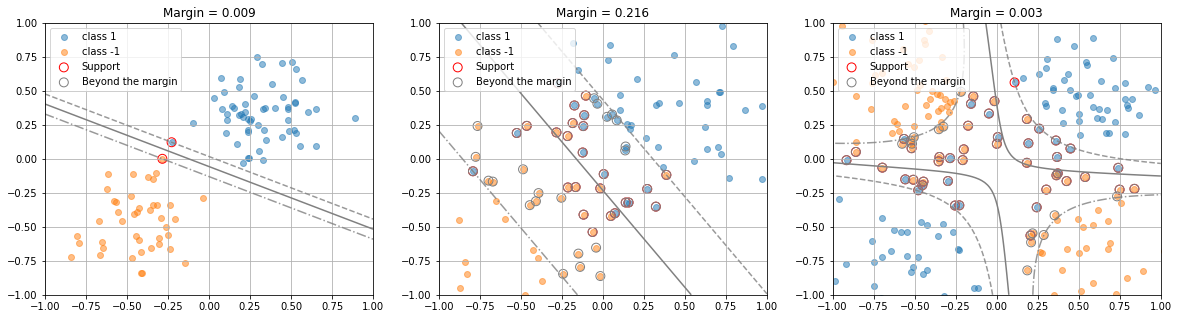
\includegraphics[width=\textwidth]{figures/classifier.png}
        \caption{Kernel Support Vector Classifier}
        \label{fig:classifier}
    \end{figure}
    \end{enumerate}
\end{enumerate}

\section{Exercise 2. Kernel Support Vector Regression}

\begin{enumerate}
\item
    \begin{enumerate}
    \item From the Representer theorem we can express $f = \sum_i \beta_i K_{x_i}$. Then the Lagrangian writes
    \begin{align*}
    &\frac{1}{2} \beta^T K \beta + C \cdot \sum_{i=1}^N \xi^+_i + \xi^-_i \\
    +& \alpha^{+T} \big ( y - K\beta - b \mathbf{1} - \eta \mathbf{1} - \xi^+ \big ) \\
    +& \alpha^{-T} \big ( -y + K\beta + b\mathbf{1} - \eta \mathbf{1} - \xi^- \big ) \\
    -& \mu^{+T} \xi^+ - \mu^{-T} \xi^-
    \end{align*}
    \item
    The Lagrangian is affine in $b$, which yields the condition $\sum_i \alpha^+_i = \sum_i \alpha^-_i $ for the dual function not to be $-\infty$.\\
    The Lagrangian is affine in $\xi^+$, which yields the condition $\forall i$, $ \alpha^+_i + \mu_i^+= C $ for the dual function not to be $-\infty$.\\
    The Lagrangian is affine in $\xi^-$, which yields the condition $\forall i$, $ \alpha^-_i + \mu_i^-= C $ for the dual function not to be $-\infty$.\\
    The Lagrangian is convex, coercive in $\beta$. As in exercise $1$, we can restrict ourselves to a single point that nullifies the gradient $\nabla_\beta L = K\beta - K (\alpha^+ - \alpha^-)$, such as $\hat{\beta} \defeq \alpha^+ - \alpha^-$.\\
    Finally, we get the Lagrange dual function
    \[ \begin{cases}
        - \frac{1}{2}(\alpha^+ - \alpha^-)^T K (\alpha^+ - \alpha^-) + y^T (\alpha^+ - \alpha^-) - \eta \sum_i \alpha_i^+ + \alpha_i^- \\ \qquad \qquad \textrm{si $\sum_i \alpha^+_i = \sum_i \alpha^-_i $, $ \alpha^\pm_i + \mu_i^\pm= C $} \\
        - \infty \, \qquad \textrm{sinon}
    \end{cases} \]
    Again, the variables $\mu^\pm$ are redundant and we can express the dual problem in the sole variables $\alpha^\pm$, and by changing the signs as a minimization :
    \begin{equation*}
    \begin{aligned}
    & \underset{\alpha^+, \alpha^-}{\text{minimize}}
    & &  \frac{1}{2}(\alpha^+ - \alpha^-)^T K (\alpha^+ - \alpha^-) - y^T (\alpha^+ - \alpha^-) + \eta \sum_i \alpha_i^+ + \alpha_i^-\\
    & \text{subject to}
    & & \sum_i \alpha_i^+ = \sum_i \alpha_i^- \\
    & & & 0 \preceq \alpha^+ \preceq C\\
    & & & 0 \preceq \alpha^- \preceq C
    \end{aligned}
    \end{equation*}
    At optimal points, $\beta^*$ minimizes the Lagrangian, and as we saw earlier, we can choose without loss of generality $\beta^*_i \defeq \alpha^+_i - \alpha^-_i$. Then for a new input $x$, we have
    \[ f(x) = \sum_i (\alpha^+_i - \alpha^-_i) \K(x_i, x)
    \]
    Note that this is $K(\alpha^+ - \alpha^-)$ for the (joint) original inputs.
    \item The reasoning is similar as in exercise 1. Skipping the computations (which are not different from earlier), we have from complementary slackness conditions:\\
    \textbf{If $0 < \alpha^+_i < C$} then $y_i - f(x_i) - b = \eta$, i.e. $x_i$ is on the boundary\\
    \textbf{If $0 < \alpha^-_i < C$} then $-y_i + f(x_i) + b = \eta$, i.e. $x_i$ is on the boundary as well.\\
    Otherwise we cannot know for sure.
    \end{enumerate}
\item
    \begin{enumerate}
    \item See the full code \href{https://github.com/gbelouze/mva-kernel-hw3/blob/b57749258006dcfc57c9f2e233fad94ef4b50f47/src/hw3/models/classify.py#L137}{on Github}
    \inputminted{python}{snippets/ex2_q2a.py}
    \item See the full code \href{https://github.com/gbelouze/mva-kernel-hw3/blob/b57749258006dcfc57c9f2e233fad94ef4b50f47/src/hw3/models/classify.py#L209}{on Github}
    \inputminted{python}{snippets/ex2_q2b.py}
    \item We test our implementation on the provided dataset. The number of support vectors is
    $42$ (of course...). See \autoref{fig:regressor}.
    \begin{figure}
        \centering
        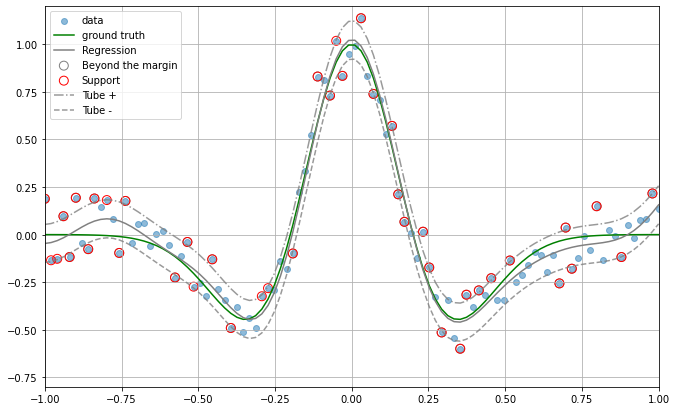
\includegraphics[width=\textwidth]{figures/regressor.png}
        \caption{Kernel Support Vector Regressor}
        \label{fig:regressor}
    \end{figure}
    \end{enumerate}
\end{enumerate}

\end{document}
